\section{Execution}
\label{sec:Durchführung}

\begin{figure}
    \centering 
    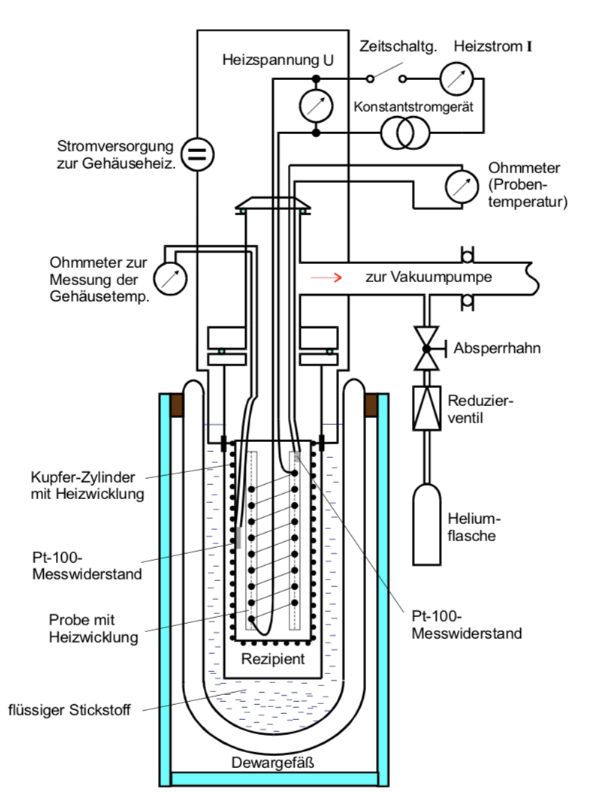
\includegraphics[width=.8\textwidth]{bilder/Aufbau.PNG}
    \caption{Experimental setup. \cite{V47}}
    \label{fig:Aufbau}
\end{figure}


The used experimental setup is shown in figure \ref{fig:Aufbau}.
At first the recipient has to be evaccuated and filled with helium gas.
The sample ($m=\SI{342}{\g}$) is surrounded by liquid nitrogen, 
to cool the sample to nearly $T=\SI{80}{\kelvin}$. 
The liquid nitrogen is filled into a cryogenic storage dewar 
and stored there throughout the whole process.
To heat up the copper to a specific temperature
a heating coil with a adjustable engergy input is used.
The added engergy depends on the current and the voltage.
To reduce heat losses through other processes like radiation or convection, 
the recipient is kept at the same temperature as the sample.
The temperature is messured indirectly by Pt-100-resistors.
To calculate the temperatures the equation
\begin{equation}
    \label{eq:T}
    T = 0.00134 R^2 + 2.296 R - 243.02
\end{equation}
is used.
$R$ is the messured resistance.




Starting by a temperature of $T=\SI{-180}{\celsius}$, the temperature is raised evenly up to $T=\SI{20}{\celsius}$. 
The resistances - representive for the temperatures-, the time, the current and the voltage are messured 
and noted for every $\SI{10}{\kelvin}$ increment.
%Was wurde gemessen bzw. welche Größen wurden variiert?